\begin{frame}{Pomodoro}
  \begin{center}
    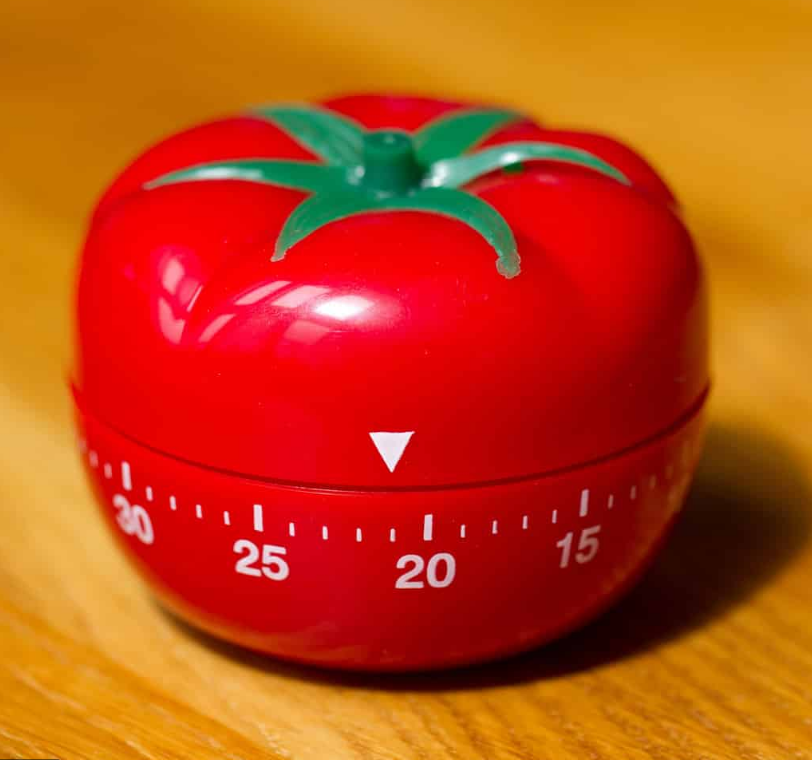
\includegraphics[height=7cm]{img/pomodoro.png}
  \end{center}
\end{frame}

\begin{frame}{Pomodoro}
  \begin{block}{Characteristics}
    \begin{itemize}
      \item Time management method.
      \item Time boxed.
      \item Iterative and incremental development.
      \item Work interval (25m) called Pomodoro.
      \item Short break (5m).
      \item 4 Pomodoros form a set, followed by a longer break (15m).
      \item Reduce interruptions.
      \item Focus and flow.
      \item Stages: planning, tracking, recording, processing and visualizing.
    \end{itemize}
  \end{block}
\end{frame}

\begin{frame}{Pomodoro}
  \begin{block}{Steps}
    \begin{itemize}
      \item Decide on the task to be done.
      \item Set the pomodoro timer (traditionally to 25 minutes).
      \item Work on the task.
      \item End work when the timer rings and put a checkmark on a piece of paper.
      \item If you have fewer than four checkmarks, take a short break (3–5 minutes) and then return to step 2; otherwise continue to step 6.
      \item After four pomodoros, take a longer break (15–30 minutes), reset your checkmark count to zero, then go to step 1.
    \end{itemize}
  \end{block}
\end{frame}

\begin{frame}{Pomodoro}
  \begin{block}{Remaining time}
    \begin{itemize}
      \item Review and edit the work just completed.
      \item Review the activities from a learning point of view: What did I learn? What could I do better or differently?
      \item Review the list of upcoming tasks for the next planned Pomodoro time blocks, and start reflecting on or updating those tasks.
    \end{itemize}
  \end{block}
\end{frame}

